\documentclass[uplatex,tikz,dvipdfmx]{standalone}

\usepackage{amsmath,amsfonts,amssymb}
\usepackage{bm}
\usepackage{siunitx}
\usepackage{standalone}
\usepackage{tikz-feynhand}

\begin{document}
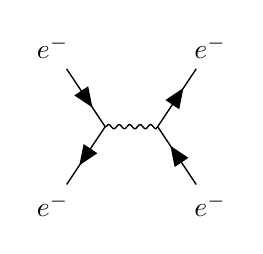
\begin{tikzpicture}
  \begin{feynhand}
    \vertex [particle] (i1) at (-1.5/1.5,1.5/1.5) {$e^-$};
    \vertex [particle] (i2) at (-1.5/1.5,-1.5/1.5) {$e^-$};
    \vertex [particle] (f1) at (1.5/1.5,1.5/1.5) {$e^-$};
    \vertex [particle] (f2) at (1.5/1.5,-1.5/1.5) {$e^-$};
    \vertex (w1) at (-0.5/1.5, 0);
    \vertex (w2) at (0.5/1.5, 0);
    \propag [boson] (w1) to (w2);
    \propag [fermion] (w2) to (f1);
    \propag [anti fermion] (w2) to (f2);
    \propag [fermion] (i1) to (w1);
    \propag [anti fermion] (i2) to (w1);
  \end{feynhand}
\end{tikzpicture}
\end{document}